\documentclass[a4paper, 9pt]{scrartcl}\usepackage[]{graphicx}\usepackage[]{xcolor}
% maxwidth is the original width if it is less than linewidth
% otherwise use linewidth (to make sure the graphics do not exceed the margin)
\makeatletter
\def\maxwidth{ %
  \ifdim\Gin@nat@width>\linewidth
    \linewidth
  \else
    \Gin@nat@width
  \fi
}
\makeatother

\definecolor{fgcolor}{rgb}{0.345, 0.345, 0.345}
\newcommand{\hlnum}[1]{\textcolor[rgb]{0.686,0.059,0.569}{#1}}%
\newcommand{\hlstr}[1]{\textcolor[rgb]{0.192,0.494,0.8}{#1}}%
\newcommand{\hlcom}[1]{\textcolor[rgb]{0.678,0.584,0.686}{\textit{#1}}}%
\newcommand{\hlopt}[1]{\textcolor[rgb]{0,0,0}{#1}}%
\newcommand{\hlstd}[1]{\textcolor[rgb]{0.345,0.345,0.345}{#1}}%
\newcommand{\hlkwa}[1]{\textcolor[rgb]{0.161,0.373,0.58}{\textbf{#1}}}%
\newcommand{\hlkwb}[1]{\textcolor[rgb]{0.69,0.353,0.396}{#1}}%
\newcommand{\hlkwc}[1]{\textcolor[rgb]{0.333,0.667,0.333}{#1}}%
\newcommand{\hlkwd}[1]{\textcolor[rgb]{0.737,0.353,0.396}{\textbf{#1}}}%
\let\hlipl\hlkwb

\usepackage{framed}
\makeatletter
\newenvironment{kframe}{%
 \def\at@end@of@kframe{}%
 \ifinner\ifhmode%
  \def\at@end@of@kframe{\end{minipage}}%
  \begin{minipage}{\columnwidth}%
 \fi\fi%
 \def\FrameCommand##1{\hskip\@totalleftmargin \hskip-\fboxsep
 \colorbox{shadecolor}{##1}\hskip-\fboxsep
     % There is no \\@totalrightmargin, so:
     \hskip-\linewidth \hskip-\@totalleftmargin \hskip\columnwidth}%
 \MakeFramed {\advance\hsize-\width
   \@totalleftmargin\z@ \linewidth\hsize
   \@setminipage}}%
 {\par\unskip\endMakeFramed%
 \at@end@of@kframe}
\makeatother

\definecolor{shadecolor}{rgb}{.97, .97, .97}
\definecolor{messagecolor}{rgb}{0, 0, 0}
\definecolor{warningcolor}{rgb}{1, 0, 1}
\definecolor{errorcolor}{rgb}{1, 0, 0}
\newenvironment{knitrout}{}{} % an empty environment to be redefined in TeX

\usepackage{alltt}
\usepackage[ngerman]{babel}
% -----------------------------------------------------------------------

% -----------------------------------------------------------------------
%% ------------------------------------------------------------
%% by J.Kruppa on Friday, February 11, 2022 (11:31)
%% \def\mainDir{\Sexpr{exam_path}}
\def\source{/Users/jokruppa/source/tex}
\usepackage[margin=2cm, includefoot]{geometry}
\setlength{\parindent}{0cm}
\usepackage{booktabs}
\usepackage{amsmath}
\usepackage{scalerel,amssymb}
\usepackage{setspace}
\def\csquare{{\Large $\boxtimes$}}
\def\msquare{{\Large $\square$}}
\usepackage[normalem]{ulem}
\usepackage{array}
\usepackage{xcolor}
\usepackage{float}
\usepackage{currfile}
\usepackage{tikz}
\usepackage[nomessages]{fp}

%% beamer defs
\def\lecture{Klausurfragen der Bio Data Science}

%% exam defs
\def\examtitle{\lecture}
\def\exammodule{
\vspace{-1.75cm}  
\begin{graybox}{}
\vspace{2Ex}
\textbf{\large Name:} \rule[0ex]{16.75em}{.4pt}
\hfill \textnormal{\textit{Nicht bestanden:}} \msquare \\[2.5Ex]
\textbf{\large Vorname:} \rule[0ex]{15em}{.4pt} \\[2.5Ex]
\textbf{\large Matrikelnummer:} \rule[0ex]{10.8em}{.4pt}
\hfill Endnote: \rule[0ex]{7em}{.4pt} 
\end{graybox}
\vspace{3Ex}
\phantom{text}
}
\def\examsemester{Sommersemester \& Wintersemester}
\def\examdate{\today}
%% ------------------------------------------------------------
\definecolor{darkblue}{rgb}{0,0,.5}
\definecolor{darkpurple}{rgb}{0.4117, 0.2, 0.4117}
\definecolor{uni}{rgb}{0,0.3137,0.6078}
\definecolor{gray}{gray}{0.7}

\usepackage{tcolorbox}
\definecolor{logo1}{RGB}{0, 158, 227}
\definecolor{gray5}{RGB}{247, 247, 247}
\definecolor{gray2}{RGB}{102, 102, 102}

\newtcolorbox{graybox}[1]{
  colback=gray5,%%red!5!white,
  colframe=gray2,%%red!75!black,
  fonttitle=\bfseries\Large,
  %%valign=center,
  fontupper=\large,
  before skip=10pt plus 2pt,
  after skip=20pt plus 4pt,
  title=#1}

\newtcolorbox{takehomebox}[1]{
  colback=gray5,%%red!5!white,
  colframe=logo1,%%red!75!black,
  fonttitle=\bfseries\Large,
  %%valign=center,
  fontupper=\large,
  before skip=10pt plus 2pt,
  after skip=10pt plus 2pt,
  title=#1}

\def\Rlogo{
\includegraphics[width = 0.5cm]{\string~/Documents/GitHub/exam/img/Rlogo}\;}

\usepackage[scaled=.90]{helvet} 
\usepackage{fancyhdr}
\usepackage{lastpage}
\usepackage{hyperref}
\hypersetup{
    colorlinks=true,       % false: boxed links; true: colored links
    linkcolor=black,          % color of internal links 
    urlcolor=magenta           % color of external links
}
\renewcommand{\familydefault}{\sfdefault}

\title{
\large \exammodule \\[5Ex]
\Huge \examtitle \\[2Ex] 
\Large Hochschule Osnabr{\"u}ck
}
\author{Pr{\"u}fer: Prof. Dr. Jochen Kruppa \\
Fakult{\"a}t f{\"u}r Agrarwissenschaften und Landschaftsarchitektur \\ 
j.kruppa@hs-osnabrueck.de}
\date{Version vom \examdate}

%% ------------------------------------------------------------
%% by J.Kruppa on Tuesday, September 23, 2014 (12:50)
%% Header
\renewcommand{\headrulewidth}{0pt}
\renewcommand{\footrulewidth}{0pt}
\pagestyle{fancy}

\fancyhf{}
\fancyhead[L]{}
\fancyhead[R]{}
\fancyfoot[R]{\thepage}
\fancyfoot[L]{\footnotesize \examtitle}

\fancypagestyle{empty}{
 \fancyhf{}
 \fancyhead[L]{}
 \fancyhead[R]{}
 \fancyfoot[R]{\thepage}
 \fancyfoot[L]{\footnotesize \examtitle}
}

\usepackage{arevtext,arevmath}

\newcommand\Tstrut{\rule{0pt}{2.6ex}}         % = `top' strut
\newcommand\Bstrut{\rule[-0.9ex]{0pt}{0pt}}   % = `bottom' strut
\def\strut{\Tstrut\Bstrut}

% -----------------------------------------------------------------------
\IfFileExists{upquote.sty}{\usepackage{upquote}}{}
\begin{document}
% -----------------------------------------------------------------------
\maketitle
\thispagestyle{empty}
\clearpage
% -----------------------------------------------------------------------

\begin{graybox}{Erlaubte Hilfsmittel f{\"u}r die Klausur}
  \vspace{1Ex}
  \begin{itemize}
  \item Normaler Taschenrechner ohne M{\"o}glichkeit der Kommunikation mit anderen
    Ger{\"a}ten - also ausdr{\"u}cklich kein Handy!
  \item Eine DIN A4-Seite als beidseitig, selbstgeschriebene,
    handschriftliche Formelsammlung - keine digitalen Ausdrucke. 
  \item \textbf{You can answer the questions in English without any consequences.}  
  \end{itemize}
\end{graybox}
\vfill

\begin{graybox}{Ergebnis der Klausur}
  \vspace{1Ex}
  \begin{itemize}
  \item[] \rule[0ex]{3em}{.4pt}\, von 20\, Punkten sind aus dem Multiple
    Choice Teil erreicht.
  \item[] \rule[0ex]{3em}{.4pt}\, von 79 Punkten sind aus dem Rechen- und
    Textteil erreicht. 
  \item[] \rule[0ex]{3em}{.4pt}\, von 99 Punkten in Summe.
  \item[] Es wird folgender Notenschl{\"u}ssel angewendet.   
  \end{itemize}
  \vspace{1ex}
\begin{center}
  \begin{tabular}[c]{cc}
    \toprule
    \textbf{Punkte}	&	\textbf{Note}	\\
    \midrule
    94.5 - 99.0	&	1,0	\\
    89.5 - 94.0	&	1,3	\\
    85.0 - 89.0	&	1,7	\\
    80.0 - 84.5	&	2,0	\\
    75.0 - 79.5	&	2,3	\\
    70.0 - 74.5	&	2,7	\\
    65.0 - 69.5	&	3,0	\\
    60.5 - 64.5	&	3,3	\\
    55.5 - 60.0	&	3,7	\\
    49.5 - 55.0	&	4,0	\\
    \bottomrule
  \end{tabular}
\end{center}
  \vspace{1ex}
\begin{itemize}
\item[] Es ergibt sich eine Endnote von \rule[0ex]{4em}{.4pt}.
\end{itemize}
  \vspace{1Ex}
\end{graybox}

% -----------------------------------------------------------------------
\newpage
% -----------------------------------------------------------------------

\begin{graybox}{Multiple Choice Aufgaben}
  \begin{itemize}
  \item Pro Multipe Choice Frage ist \emph{genau} eine Antwort richtig.
  \item \textbf{Übertragen Sie Ihre Kreuze in die Tabelle auf
      dieser Seite.}
  \item Es werden nur Antworten berücksichtigt, die in dieser Tabelle
    angekreuzt sind!
  \end{itemize}

\begin{center}
  \large
  \begin{tabular}{|r|c|c|c|c|c||c|}
    \hline
    & \textbf{A} & \textbf{B} & \textbf{C} & \textbf{D} & \textbf{E} & $\boldsymbol{\checkmark}$\strut\\
    \hline
    1 Aufgabe &   &   &   &   &   & \strut\\
    \hline
    2 Aufgabe &   &   &   &   &   & \strut\\
    \hline
    3 Aufgabe &   &   &   &   &   & \strut\\
    \hline
    4 Aufgabe &   &   &   &   &   & \strut\\
    \hline
    5 Aufgabe &   &   &   &   &   & \strut\\
    \hline
    6 Aufgabe &   &   &   &   &   & \strut\\
    \hline
    7 Aufgabe &   &   &   &   &   & \strut\\
    \hline
    8 Aufgabe &   &   &   &   &   & \strut\\
    \hline
    9 Aufgabe &   &   &   &   &   & \strut\\
    \hline
    10 Aufgabe &   &   &   &   &   & \strut\\
    \hline
  \end{tabular}
\end{center}

\begin{itemize}
\item Es sind \rule[0ex]{2em}{.4pt}\, von 20 Punkten erreicht worden.
\end{itemize}
\end{graybox}

\vfill

\begin{graybox}{Rechen- und Textaufgaben}
  \begin{itemize}
  \item Die Tabelle wird vom Dozenten ausgefüllt.
  \end{itemize}
  \begin{center}
    \large
    \begin{tabular}{|l|c|c|c|c|c|c|c|}
      \hline
      \textbf{Aufgabe} & 11 & 12 & 13 & 14 & 15 & 16 & 17 \strut\\
      \hline
      \textbf{Punkte} & 
      \hspace{1Ex}\Large\textcolor{gray!70}{10}\hspace{1Ex}  & 
      \hspace{1Ex}\Large\textcolor{gray!70}{20}\hspace{1Ex}  & 
      \hspace{1Ex}\Large\textcolor{gray!70}{8}\hspace{1Ex}  & 
      \hspace{1Ex}\Large\textcolor{gray!70}{10}\hspace{1Ex}  & 
      \hspace{1Ex}\Large\textcolor{gray!70}{11}\hspace{1Ex}  & 
      \hspace{1Ex}\Large\textcolor{gray!70}{10}\hspace{1Ex}  & 
      \hspace{1Ex}\Large\textcolor{gray!70}{10}\hspace{1Ex} \strut\\
      \hline
  \end{tabular}
\end{center}
\begin{itemize}
\item Es sind \rule[0ex]{2em}{.4pt}\, von 79 Punkten erreicht worden.
\end{itemize}
\end{graybox}

% -----------------------------------------------------------------------
\clearpage
% -----------------------------------------------------------------------


\section{Aufgabe \hfill (2 Punkte)}

%% --------------------------------------------------------------------
\ifcollection
\begin{flushright}
\tiny\vspace{-2Ex}
\textbf{\examinhaltstart}
\exammodulestatversuch $\;\bullet$
\exammodulebiostat
\vspace{-1Ex}
\end{flushright}
\fi
%% --------------------------------------------------------------------




Ein Versuch wurde an 65 Tieren durchgeführt, wobei jedes Tier eine von drei Vitamin-C-Dosen (0.5, 1 und 1.5 mg/Tag) über eine von zwei Verabreichungsmethoden erhielt. Die folgende Abbildung enthält die Daten aus diesem Versuch zur Bewertung der Wirkung von Vitamin E auf das Zahnwachstum bei Hasen.  Welche Aussage ist richtig, wenn Sie eine zweifaktorielle ANOVA rechnen?



{\centering 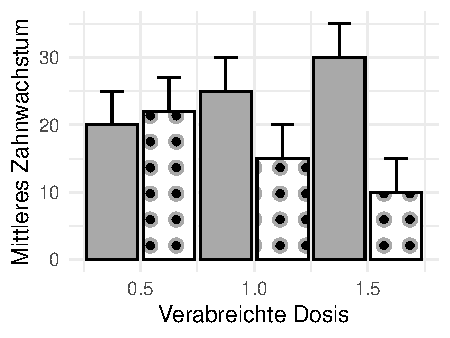
\includegraphics[width=\maxwidth]{img/mc-anova-02-a-1} 

}







\begin{enumerate}
\item [\textbf{A} \msquare] Keine Interaktion liegt vor $(p \leq 0.05)$.
\item [\textbf{B} \msquare] Das Bestimmtheitsmaß $R^2$ ist groß.
\item [\textbf{C} \msquare] Mit $(p \leq 0.05)$ liegt eine mittlere bis starke Interaktion vor.
\item [\textbf{D} \msquare] Die Koeffizienten sind positiv $(\beta_0 > 0; \beta_1 > 0)$.
\item [\textbf{E} \msquare] Das Bestimmtheitsmaß $R^2$ ist klein.
\end{enumerate} 

\section{Aufgabe \hfill (2 Punkte)}

%% --------------------------------------------------------------------
\ifcollection
\begin{flushright}
\tiny\vspace{-2Ex}
\textbf{\examinhaltstart}
\exammodulemathstat $\;\bullet$
\exammodulestat $\;\bullet$
\exammodulestatbbv $\;\bullet$
\exammodulestatversuch $\;\bullet$
\exammodulebiostat
\vspace{-1Ex}
\end{flushright}
\fi
%% --------------------------------------------------------------------



In Ihrer Abschlussarbeit wollen Sie zu Beginn eine explorativen Datenanalyse (EDA) in \Rlogo rechnen. Dafür gibt es eine generelle Abfolge von Prozessschritten. Welche ist hierbei die richtige Reihenfolge?



\begin{enumerate}
\item [\textbf{A} \msquare] Wir lesen die Daten ein und mutieren die Daten. Dabei ist wichtig, dass wir nicht das Paket \texttt{tidyverse} nutzen, da dieses Paket veraltet ist. über die Funktion \texttt{library(tidyverse)} entfernen wir das Paket von der Analyse.
\item [\textbf{B} \msquare] Wir lesen als erstes die Daten über \texttt{read\_excel()} ein, transformieren die Spalten über \texttt{mutate()} in die richtige Form und können dann über \text{ggplot()} uns die Abbildungen erstellen lassen.
\item [\textbf{C} \msquare] Wir lesen als erstes die Daten über \texttt{read\_excel()} ein, transformieren die Spalten über \texttt{mutate()} in die richtige Form und können dann  über \text{ggplot()} uns die Abbildungen erstellen lassen. Wichtig ist, dass wir keine Faktoren sondern nur numerische Variablen vorliegen haben.
\item [\textbf{D} \msquare] Für eine explorativen Datenanalyse (EDA) in \Rlogo müssen wir als erstes die Daten über \texttt{read\_excel()} einlesen. Danach müssen wir schauen, dass wir die Zeilen richtig über \texttt{mutate()} transformiert haben. Insbesondere müssen Variablen mit kontinuierlichen Werten in einen Faktor umgewandelt werden. Am Ende nutzen wir die Funktion \text{ggplot()} für die eigentlich EDA.
\item [\textbf{E} \msquare] Wir lesen die Daten über eine generische Funktion \texttt{read()} ein und müssen dann die Funktion \texttt{ggplot()} nur noch installieren. Dann haben wir die Abbildungen als \texttt{*.png} vorliegen.
\end{enumerate} 

\section{Aufgabe \hfill (2 Punkte)}

%% --------------------------------------------------------------------
\ifcollection
\begin{flushright}
\tiny\vspace{-2Ex}
\textbf{\examinhaltstart}
\exammodulestatversuch $\;\bullet$
\exammodulebiostat
\vspace{-1Ex}
\end{flushright}
\fi
%% --------------------------------------------------------------------




Der multiple Vergleich als Posthoc-Test nach einer ANOVA ist in den Agrarwissenschaften heutzutage Standard. Welches R Paket wird häufig für den multiplen Vergleich genutzt? Welche Beschreibung der Eigenschaften ist korrekt?



\begin{enumerate}
\item [\textbf{A} \msquare] Das R Paket \{lm\}. Das Paket \{lm\} erstellt selbstständig Konfidenzintervalle und entsprechende p-Werte. Da wir in dem Paket nicht adjustieren müssen, ist es bei Anwendern sehr beliebt.
\item [\textbf{B} \msquare] Das R Paket \{ggplot\}. Wir erhalten hier sofort eine Visualisierung der Daten. Anhand der Visualisierung lässt sich eine explorative Datenanalyse durchführen, die gleichwertig zu einem Posthoc-Test ist.
\item [\textbf{C} \msquare] Das R Paket \{hmisc\} erlaubt die Durchführung eines multiplen Gruppenvergleichs aus verschiedenen Modellen heraus. Aus einem hmisc Objekt lässt sich recht einfach das CLD erstellen und so über Barplots eine schnelle Interpration der statistischen Auswertung durchführen.
\item [\textbf{D} \msquare] Das R Paket \{emmeans\} erlaubt die Durchführung eines multiplen Gruppenvergleichs. Aus einem \{emmeans\} Objekt lässt sich recht einfach das CLD erstellen und so über Barplots eine schnelle Interpration der statistischen Auswertung durchführen.
\item [\textbf{E} \msquare] Das R Paket \{emmeans\} erlaubt die Durchführung eines multiplen Gruppenvergleichs. Aus einem emmeans Objekt lässt sich leider kein CLD erstellen. Dennoch ist das Paket einfach zu bedienen und wird deshalb genutzt. Die Interpretation der statistischen Auswertung wird über einen Barplot abgebildet.
\end{enumerate} 

\section{Aufgabe \hfill (2 Punkte)}

%% --------------------------------------------------------------------
\ifcollection
\begin{flushright}
\tiny\vspace{-2Ex}
\textbf{\examinhaltstart}
\exammodulebiostat
\vspace{-1Ex}
\end{flushright}
\fi
%% --------------------------------------------------------------------




Sie haben ein Feldexperiment mit Erbsen durchgeführt und wollen nun in einer simplen linearen Regression den Einfluss der $CO_2$-Konzentration in [$\mu g$] im Wasser auf den absoluten Proteingehalt in [$kg$] untersuchen. Sie erhalten einen $\beta_{CO_2}$ Koeffizienten von $6.9\times 10^{-7}$ und einen $p$-Wert mit $0.00032$. Welche Aussage zu der Signifikanz und dem Effekt ist richtig?




\begin{enumerate}
\item [\textbf{A} \msquare] Die Fallzahl ist zu hoch angesetzt. Je höher die Fallzahl ist, desto kleiner ist die Teststatistik und damit ist dann auch der $p$-Wert sehr klein. Es sollte über eine Reduzierung der Fallzahl nachgedacht werden. Dann sollte der Effekt zum p-Wert passen.
\item [\textbf{B} \msquare] Wenn der Effekt $\beta_{CO_2}$ sehr klein ist, dann kann es an einer falsch gewählten Einheit liegen. Der Anstieg von einer Einheit in $X$ führt ja zu einer Änderung von $\beta_{CO_2}$ in $y$. Daher ist hier mit einer anderen Einheit in den Daten zu rechnen, so dass wir hier einen besser formatierten Effekt sehen. Der p-Wert stammt aus einer einheitslosen Teststatistik.
\item [\textbf{C} \msquare] Manchmal ist die Einheit der Einflussvariable $X$ zu groß gewählt, so dass der Ansteig von 1 Einheit in $X$ zu einer zu großen Änderung in $y$ führt. Daher kann der Effekt $\beta_{CO_2}$ sehr klein wirken, da der p-Wert wird auf einer einheitslosen Teststatistik bestimmt wird.
\item [\textbf{D} \msquare] Das Gewicht und die $CO_2$-Konzentration korrelieren sehr stark, deshalb wird der $\beta_{CO_2}$ Koeffizient sehr klein. Mit einer ANOVA kann für die Korrelation korrigiert werden und der Effektschätzer passt dann zum p-Wert.
\item [\textbf{E} \msquare] Die Einheit der $CO_2$-Konzentration ist zu klein gewählt. Dadurch sehen wir den sehr kleinen $p$-Wert. Der $p$-Wert und die Einheit von der $CO_2$-Konzentration hängen antiproportional zusammen.
\end{enumerate} 

\section{Aufgabe \hfill (2 Punkte)}

%% --------------------------------------------------------------------
\ifcollection
\begin{flushright}
\tiny\vspace{-2Ex}
\textbf{\examinhaltstart}
\exammodulestatversuch $\;\bullet$
\exammodulebiostat
\vspace{-1Ex}
\end{flushright}
\fi
%% --------------------------------------------------------------------






Sie rechnen einen statistischen Test und wollen anhand des 95\%-Konfidenzintervalls eine Entscheidung gegen die Nullhypothese treffen. Welche Aussage ist richtig?





\begin{enumerate}
\item [\textbf{A} \msquare] Anhand des 95\%-Konfidenzintervalls lässt sich wie folgt eine Entscheidung treffen. Ist der Wert kleiner dem Signifikanzniveau $\alpha$ dann kann die Nullhypothese abgelehnt werden.
\item [\textbf{B} \msquare] Anhand des 95\%-Konfidenzintervalls lässt sich wie folgt eine Entscheidung treffen. Liegt der Wert in dem Signifikanzniveauintervall $\alpha$ dann kann die Nullhypothese abgelehnt werden.
\item [\textbf{C} \msquare] Das Signifikanzniveauintervall $\alpha$ ist gleich $5\%$ und damit muss das berechnete Intervall unter dem Signifikanzniveauintervall $\alpha$ liegen, dann kann die Nullhypothese nicht abgelehnt werden.
\item [\textbf{D} \msquare] Wir betrachten das Ganze Intervall des 95\%-Konfidenzintervalls. Liegt die Null mit in dem Intervall, dann kann die Nullhypothese abgelehnt werden.
\item [\textbf{E} \msquare] Der kritische Wert $T_{\alpha = 5\%}$ ist tabelarisch festgelegt und gegeben. Ist $T_{D}$ größer als der kritische Wert, kann die Nullhypothese abgelehnt werden
\end{enumerate} 

\section{Aufgabe \hfill (2 Punkte)}


%% --------------------------------------------------------------------
\ifcollection
\begin{flushright}
\tiny\vspace{-2Ex}
\textbf{\examinhaltstart}
\exammodulestatversuch $\;\bullet$
\exammodulebiostat
\vspace{-1Ex}
\end{flushright}
\fi
%% --------------------------------------------------------------------




Um zu Überprüfen, ob die Daten die Annahme einer Varianzhomogenität genügen, können wir folgende Visualisierung nutzen. Dabei kommt dann auch die entsprechende Regel zur Abschätzung der Annahme einer Varianzhomogenität zur Anwendung.



\begin{enumerate}
\item [\textbf{A} \msquare] Nach der Erstellung eines Boxplots schauen wir, ob der Median in der Mitte der Box liegt. Dabei ist der Median als dicke Linie dargestellt und die Box ist das IQR.
\item [\textbf{B} \msquare] Einen Boxplot. Das IQR muss über alle Behandlungen zusammen mit den Whiskers ungefähr gleich aussehen.
\item [\textbf{C} \msquare] Einen Barplot. Die Mittelwerte müssen alle auf einer Höhe liegen. Die Fehlerbalken haben hier keine Informationen.
\item [\textbf{D} \msquare] Einen Dotplot. Die Punkte müssen sich wie an einer Perlenschnurr audreihen. Eine Abweichung führt zur Ablehnung der Annahme einer Varianzhomogenität.
\item [\textbf{E} \msquare] In einer explorativen Datanalyse nutzen wir den Violinplot. Dabei sollte der Bauch am Rand liegen. Dann können wir von einer Varianzhomogenität ausgehen.
\end{enumerate} 

\section{Aufgabe \hfill (2 Punkte)}

%% --------------------------------------------------------------------
\ifcollection
\begin{flushright}
\tiny\vspace{-2Ex}
\textbf{\examinhaltstart}
\exammodulebiostat
\vspace{-1Ex}
\end{flushright}
\fi
%% --------------------------------------------------------------------




Neben der Mittelwertsdifferenz als Effektschätzer bei normalverteilten Endpunkten wird auch häufig der Effektschätzer Risk ratio bei binären Endpunkten verwendet. Welche Aussage über den Effektschätzer Risk ratio ist im folgenden Beispiel zur Behandlung von Klaueninfektionen bei Schweinen richtig? Dabei sind 3 Tiere krank und 12 Tiere sind gesund.



\begin{enumerate}
\item [\textbf{A} \msquare] Es ergibt sich ein Risk ratio von 4, da es sich um ein Anteil handelt.
\item [\textbf{B} \msquare] Das Verhältnis von Chancen Risk ratio ergibt ein Chancenverhältnis von 0.25.
\item [\textbf{C} \msquare] Da es sich um ein Chancenverhältnis handelt ergibt sich ein Risk ratio von 5.
\item [\textbf{D} \msquare] Es ergibt sich ein Risk ratio von 0.25, da es sich um ein Anteil handelt.
\item [\textbf{E} \msquare] Der Anteil der Kranken wird berechnet. Da es sich um ein Anteil handelt ergibt sich ein Risk ratio von 0.2.
\end{enumerate} 

\section{Aufgabe \hfill (2 Punkte)}

%% --------------------------------------------------------------------
\ifcollection
\begin{flushright}
\tiny\vspace{-2Ex}
\textbf{\examinhaltstart}
\exammodulestatversuch $\;\bullet$
\exammodulebiostat
\vspace{-1Ex}
\end{flushright}
\fi
%% --------------------------------------------------------------------




Sie führen paarweise t-Tests für alle Vergleiche der verschiedenen Rapssorten in Ihrem Experiment durch. Nach der Adjustierung für multiples Testen ist kein p-Wert unter der $\alpha$-Schwelle. Ihr Experiment beinhaltet fünf Rapssorten und eine ANOVA ergibt $p = 0.045$ für den Ertrag. Sie schauen sich auch die rohen, unadjustierten p-Werte an und finden hier als niedrigsten p-Wert $p_{3-2} = 0.052$. Welche Aussage ist richtig?




\begin{enumerate}
\item [\textbf{A} \msquare] Der Fehler liegt in den t-Tests. Wenn eine ANOVA signifikant ist, dann muss zwangsweise auch ein t-Test signifikant sein.
\item [\textbf{B} \msquare] Die ANOVA testet auf der gesamten Fallzahl. Es wäre besser die ANOVA auf der gleichen Fallzahl wie die einzelnen t-Tests zu rechnen.
\item [\textbf{C} \msquare] Es gibt einen Fehler in der Varianzstruktur. Daher kann die ANOVA nicht richtig sein und paarweise t-Tests liefern das richtige Ergebnis.
\item [\textbf{D} \msquare] Die ANOVA testet auf der gesamten Fallzahl. Die einzelnen t-Tests immer nur auf einer kleineren Subgruppe. Da mit weniger Fallzahl weniger signifikante Ergebnisse zu erwarten sind, kann eine Diskrepenz zwischen der ANOVA und den paarweisen t-Tests auftreten.
\item [\textbf{E} \msquare] Das Beispiel kann so nicht auftreten, da die ANOVA und die t-Tests algorithmisch miteinander verschränkt sind.
\end{enumerate}

\section{Aufgabe \hfill (2 Punkte)}

%% --------------------------------------------------------------------
\ifcollection
\begin{flushright}
\tiny\vspace{-2Ex}
\textbf{\examinhaltstart}
\exammodulebiostat
\vspace{-1Ex}
\end{flushright}
\fi
%% --------------------------------------------------------------------




Welche Aussage über die \textit{Power} ist richtig?



\begin{enumerate}
\item [\textbf{A} \msquare] Die Power wird berechnet und ist keine Eigenschaft des Tests. Die Power wird auf $80\%$ gesetzt und beschreibt mit welcher Wahrscheinlichkeit $H_0$ \textit{bewiesen wird}
\item [\textbf{B} \msquare] Die Power ist nicht in der aktuellen Testthorie mehr vertreten. Wir rechnen nur noch mit dem Fehler 1. Art.
\item [\textbf{C} \msquare] Die Power wird nicht berechnet sondern ist eine Eigenschaft des Tests. Die Power wird auf $80\%$ gesetzt und beschreibt mit welcher Wahrscheinlichkeit $H_A$ \textit{bewiesen wird}
\item [\textbf{D} \msquare] Alle statistischen Tests sind so konstruiert, dass die $H_A$ mit 20\% \textit{bewiesen wird}. Die Power ist $1-\beta$ mit $\beta$ gleich 80\% gesetzt.
\item [\textbf{E} \msquare] Die Power beschreibt die Wahrscheinlichkeit die $H_A$ abzulehnen. Wir testen die Power jedoch nicht.
\end{enumerate} 

\section{Aufgabe \hfill (2 Punkte)}

%% --------------------------------------------------------------------
\ifcollection
\begin{flushright}
\tiny\vspace{-2Ex}
\textbf{\examinhaltstart}
\exammodulestat $\;\bullet$
\exammodulestatbbv $\;\bullet$
\exammodulestatversuch $\;\bullet$
\exammodulebiostat
\vspace{-1Ex}
\end{flushright}
\fi
%% --------------------------------------------------------------------




Die Normalverteilung wird durch den Mittelwert und die Standardabweichung definiert. Welche Aussage im Bezug zur Standardabweichung in einer Normalverteilung ist richtig?



{\centering 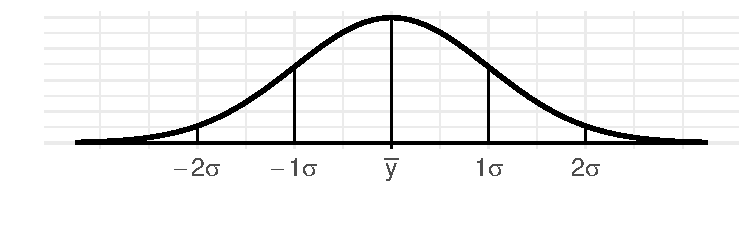
\includegraphics[width=\maxwidth]{img/mc-distribution-02-a-1} 

}







\begin{enumerate}
\item [\textbf{A} \msquare] Die Fläche unter der Kurve ist 1, wenn die Nullhypothese falsch ist. Wenn die Nullhypothese gilt, dann ist die Fläche $1-\alpha$. Somit ergibt sich auch eine Standardabweichung $\sigma$ mit $\alpha$ gleich 0.05 in beiden Fällen.
\item [\textbf{B} \msquare] Die Fläche links von $-2\sigma$ ist der p-Wert mit $Pr(D|H_0)$ in der obigen Abbildung.
\item [\textbf{C} \msquare] Die Fläche unter der Kurve entspricht dem Signifikanzniveau $\alpha$ von 5\%. Damit ist die Standardabweichung $\sigma$ gleich 1 in der obigen Abbildung.
\item [\textbf{D} \msquare] Die Fläche zwischen $-1\sigma$ und $1\sigma$ ist 0.95 und 95\% der Beobachtungen liegen somit zwischen $\bar{y}\pm\sigma$ in der obigen Verteilung.
\item [\textbf{E} \msquare] Es liegen 95\% der Beobachtungen zwischen $\bar{y}\pm 2 \sigma$. Angezeigt durch die Fläche zwischen $-2\sigma$ und $2\sigma$ in der obigen Verteilung.
\end{enumerate}

% -----------------------------------------------------------------------
\clearpage
% -----------------------------------------------------------------------

\section{Aufgabe \hfill (10 Punkte)}

\textit{Geben Sie grundsätzlich Formeln und Rechenweg zur Lösung der Teilaufgaben mit an!} \\[1Ex]
 

 
%% --------------------------------------------------------------------
\ifcollection
\begin{flushright}
\tiny\vspace{-3Ex}
\textbf{\examinhaltstart}
\exammodulestatversuch $\;\bullet$
\exammodulebiostat
\vspace{-4Ex}
\end{flushright}
\begin{minipage}[t]{0.5\textwidth}

\includegraphics[width = 1.3cm]{/Users/kruppajo/work/GitHub/exam/avatare/Jonas.png}\hspace{-4mm}
\includegraphics[width = 1.3cm]{/Users/kruppajo/work/GitHub/exam/avatare/Paula.png}
\end{minipage}
\begin{minipage}[t]{0.5\textwidth}
\hfill
\href{https://youtu.be/Op-gjzASH9I}{
\includegraphics[width = 2cm]{img/youtube}}
\end{minipage}
\fi
%% --------------------------------------------------------------------



\ifcollection
\paragraph{Visualisierung von Verteilungen}
\fi

'Ich glaube, dass es sich hier wieder um so ein kryptisches Lernziel handelt, was nicht so gleich klar ist.', meint Paula und streichelt sanft die Ratte. Das Tier versucht dem strammen Griff zu entkommen, gibt aber auf. Jonas sieht sich sehr genau die drei liegenden Boxplots an. 'Du weißt doch wie es heißt, \textit{Frei ist, wer missfallen kann.}\footnote{Oschmann, A. (2024) Mädchen stärken: Stärken fördern, Selbstwert erhöhen und liebevoll durch Krisen begleiten. Goldegg Verlag}', merkt Paula nickend an. Das Ziel ist es zu verstehen, wie eine Verteilung anhand eines Boxplots bewertet werden kann. Paula und der Perfektionismus machen die Sache nicht einfacher.



{\centering 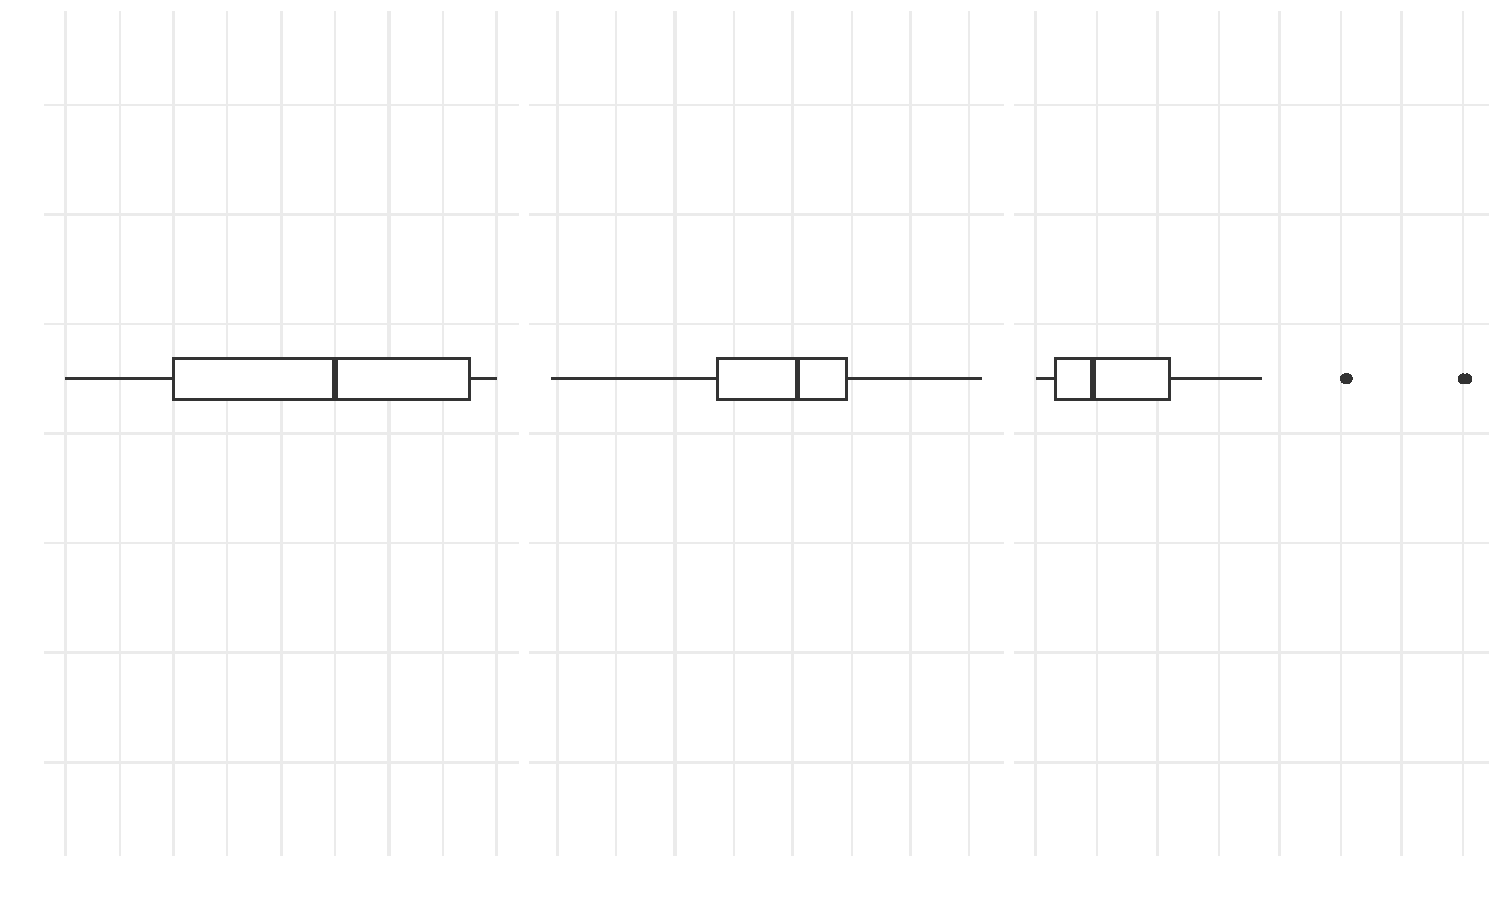
\includegraphics[width=\maxwidth]{img/desc-stat-11-1} 

}




Jetzt brauchen Paula und Jonas Ihre Hilfe bei der Abschätzung einer Verteilung anhand von Boxplots um ihre Arbeit dann in diesem Semester noch abschließen zu können.

\begin{enumerate}
\item Zeichnen Sie über die Boxplots die entsprechende zugehörige Verteilung! \textbf{(3 Punkte)} 
\item Zeichnen Sie unter die Boxplots die entsprechende zugehörige Beobachtungen als Stiche! \textbf{(3 Punkte)}
\item Wie viel Prozent der Beobachtungen fallen in das IQR? Ergänzen Sie die Abbildung entsprechend um den Bereich! \textbf{(2 Punkte)}
\item Wie viel Prozent der Beobachtungen fallen in $\bar{y} \pm 1s$ und $\bar{y} \pm 2s$  unter der Annahme einer Normalverteilung? \textbf{(2 Punkte)}
\end{enumerate} 
\clearpage
% -----------------------------------------------------------------------

\section{Aufgabe \hfill (20 Punkte)}

\textit{Geben Sie grundsätzlich Formeln und Rechenweg zur Lösung der Teilaufgaben mit an!} \\[1Ex]
 

 
%% --------------------------------------------------------------------
\ifcollection
\begin{flushright}
\tiny\vspace{-3Ex}
\textbf{\examinhaltstart}
\exammodulebiostat
\vspace{-4Ex}
\end{flushright}
\begin{minipage}[t]{0.5\textwidth}

\includegraphics[width = 1.3cm]{/Users/kruppajo/work/GitHub/exam/avatare/Mark.png}
\end{minipage}
\begin{minipage}[t]{0.5\textwidth}
\hfill
\href{https://youtu.be/C9skfFRTHhI}{
\includegraphics[width = 2cm]{img/caution}}
\end{minipage}
\fi
%% --------------------------------------------------------------------



\ifcollection
\paragraph{Zerforschen eines wissenschaftlichen Datensatzes}
\fi

Unter einem langen Schnaufen starrt Mark auf den wissenschaftlichen Datensatz \textit{in der Tabelle 1} in seinem Laptop. Insgesamt wurden $n$ Beobachtungen erhoben. 'Worum geht es denn eigentlich in diesem Datensatz?', fragt er sich kopfschüttelnd und mampft noch ein paar Marzipankugeln. Mark soll die Datentabelle nutzen um das eigene Experiment zu planen und eine Blaupause zu haben. Als eine Vorlage sozusagen, die er nur noch ausfüllen muss. Daher möchte seine Betreuerin, dass er einmal die Daten sinnvoll zusammenfasst. Das sollte dann doch etwas aufwendiger werden. Das wird dann vermutlich heute Abend nichts mehr mit Columbo.

\begin{table}[h]
\centering
\Large
  \begin{tabular}{ccccc}
  \toprule
   $\boldsymbol{f_1}$  & $\boldsymbol{f_2}$ & $\boldsymbol{x_1}$ & $\boldsymbol{y_1}$ & $\boldsymbol{y_2}$ \\[2pt]
     <\phantom{xxx}>  & <\phantom{xxx}> & <\phantom{xxx}> & <\phantom{xxx}> & <\phantom{xxx}> \\[2pt] 
  \midrule
  1  & 1 & 2.3 & 10.1 & 0 \\  
  1  & 1 & 4.1 & 13.1 & 0 \\ 
  1  & 1 & 5.7 & 16.5 & 1 \\ 
  1  & 1 & 3.4 & 14.6 & 0 \\
  1  & 2 & 2.8 & 12.1 & 1 \\
  1  & 2 & 6.1 & 13.4 & 1 \\
  $\vdots$  & $\vdots$ & $\vdots$ & $\vdots$ & $\vdots$\\
  1 & 2  & 1.9 & 9.6 &  0\\
  \bottomrule
  \end{tabular}
\end{table}

Mark füllt sich mit der Analyse der Daten in der Tabelle 1 überfordert. Deshalb braucht er bei der Auswertung Ihre Hilfe! Glücklicherweise kennen Sie den wissenschaftlichen Datensatz aus Ihren eigenen Analysen schon im Detail und können sofort helfen.

\begin{graybox}{}
\begin{center}
\textit{Beantworten Sie die folgenden Fragen anhand eines selbst gewählten Beispiels!}
\end{center}
\end{graybox}

\paragraph{Allgemeiner Aufgabenteil} 

\begin{enumerate}
  \setcounter{enumi}{0}
  \item Ergänzen Sie die Eigenschaften der Spalten in der Form eines \texttt{tibbles}! \textbf{(2 Punkte)}
  \item Skizzieren Sie die übergeordneten Analysebereiche der Statistik passend zur obigen Datentabelle! Beschriften Sie die Abbildungen! \textbf{(4 Punkte)}
  \item Formulieren Sie zwei mögliche wissenschaftliche Fragestellungen in Form einer PowerPoint Folie aus der obigen Datentablle! \textbf{(2 Punkte)}
\end{enumerate}

\paragraph{Spezieller Aufgabenteil für die Variablen $\boldsymbol{x_1}$ und $\boldsymbol{y_2}$}

\begin{enumerate}
  \setcounter{enumi}{3}
  \item In welchen der übergeordneten Analysebereiche der Statistik gehört die Auswertung Ihres Endpunktes? Begründen Sie Ihre Antwort! \textbf{(2 Punkte)}
  \item Skizzieren Sie eine ikonische Abbildung für Ihren Endpunkt im Kontext der wissenschaftlichen Fragestellung! \textbf{(2 Punkte)}
  \item Erstellen Sie das statistische Modell in der in \Rlogo üblichen Schreibweise! \textbf{(1 Punkt)}
  \item Skizzieren Sie die Datenanalyse für Ihren Endpunkt! \textbf{(4 Punkte)}
  \item Auf welche Eigenschaft der Daten müssen Sie für Ihre statistische Analyse im Besonderen achten? Erklären Sie eine mögliche Lösung in der Modellierung! Begründen Sie Ihre Antwort! \textbf{(2 Punkte)}
  \item Welche statistische Maßzahlen können Sie berichten? Begründen Sie Ihre Antwort! \textbf{(1 Punkt)}
\end{enumerate}

 
\clearpage
% -----------------------------------------------------------------------

\section{Aufgabe \hfill (8 Punkte)}

\textit{Geben Sie grundsätzlich Formeln und Rechenweg zur Lösung der Teilaufgaben mit an!} \\[1Ex]
 

 
%% --------------------------------------------------------------------
\ifcollection
\begin{flushright}
\tiny\vspace{-3Ex}
\textbf{\examinhaltstart}
\exammodulemathstat $\;\bullet$
\exammodulestat $\;\bullet$
\exammodulestatbbv $\;\bullet$
\exammodulestatversuch $\;\bullet$
\exammodulebiostat
\vspace{-4Ex}
\end{flushright}
\begin{minipage}[t]{0.5\textwidth}

\includegraphics[width = 1.3cm]{/Users/kruppajo/work/GitHub/exam/avatare/Mark.png}
\end{minipage}
\begin{minipage}[t]{0.5\textwidth}
\hfill
\href{https://youtu.be/t0WYa_LVc5o}{
\includegraphics[width = 2cm]{img/youtube}}
\end{minipage}
\vspace{-3ex}
\fi
%% --------------------------------------------------------------------



\ifcollection
\paragraph{Zerforschen des Barplots}
\fi

Barplots sind bedeutend in der Darstellung von wissenschaftlichen Ergebnissen. Leider hat sich Mark nicht gemerkt, welche statistischen Maßzahlen für einen Barplot erhoben werden müssen. Besser wäre was anderes gewesen. Mark liebt Geocaching. Darin kann er sich wirklich verlieren und immer wieder neu begeistern. Das ist in soweit doof, da nach seiner Betreuer erstmal ein Barplot nachgebaut werden soll, bevor es mit seiner Hausarbeit losgeht. Dann hat er schonmal den \Rlogo Code vorliegen und nachher geht dann alles schneller. Na dann mal los. Mark schafft sich die nötige Stimmung. Mark streichelt liebevoll der Hamster. Der Kopf ist in seinem Schloß vergraben um den Klang von Andrea Berg zu dämpfen. In der Behandlung für Brokoli werden verschiedene Düngestufen ($ctrl$, $low$ und $high$) sein. Erfasst wird als Outcome ($Y$) \textit{Proteingehalt}. Mark soll dann \textit{protein} in seiner Exceldatei eintragen.



{\centering 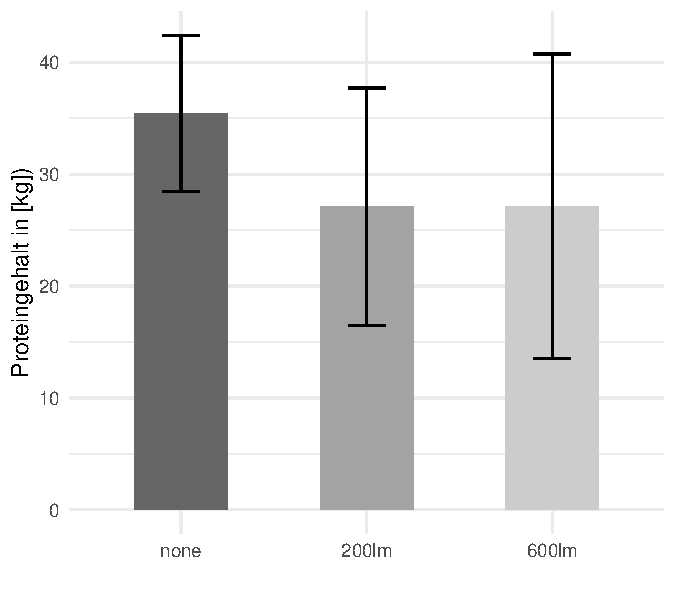
\includegraphics[width=\maxwidth]{img/barplot-02-1} 

}




Leider kennt sich Mark mit der Erstellung von Barplots in \Rlogo nicht aus. Deshalb braucht er bei der Visualisierung Ihre Hilfe!

\begin{enumerate}
\item Formulieren Sie die wissenschaftliche Fragestellung! \textbf{(1 Punkt)}
\item Erstellen Sie eine Tabelle mit den statistischen Maßzahlen der drei Barplots! \textit{Beachten Sie die korrekte Darstellungsform der statistischen Maßzahlen!} \textbf{(3 Punkte)}
\item Erstellen Sie einen beispielhaften Datensatz im \Rlogo üblichen Format, aus dem die drei Barplots \textit{möglicherweise} erstellt wurden! \textbf{(2 Punkte)}
\item Kann Mark einen Unterschied zwischen den Behandlungen erwarten? Begründen Sie Ihre Antwort! \textbf{(2 Punkte)}
\end{enumerate} 
\clearpage
% -----------------------------------------------------------------------

\section{Aufgabe \hfill (10 Punkte)}

\textit{Geben Sie grundsätzlich Formeln und Rechenweg zur Lösung der Teilaufgaben mit an!} \\[1Ex]
 

 
%% --------------------------------------------------------------------
\ifcollection
\begin{flushright}
\tiny\vspace{-3Ex}
\textbf{\examinhaltstart}
\exammodulestat $\;\bullet$
\exammodulestatbbv $\;\bullet$
\exammodulestatversuch $\;\bullet$
\exammodulebiostat
\vspace{-4Ex}
\end{flushright}
\begin{minipage}[t]{0.5\textwidth}

\includegraphics[width = 1.3cm]{/Users/kruppajo/work/GitHub/exam/avatare/Yuki.png}
\end{minipage}
\begin{minipage}[t]{0.5\textwidth}
\hfill
\href{https://youtu.be/xq29O8qDrg0}{
\includegraphics[width = 2cm]{img/youtube}}
\end{minipage}
\vspace{-3ex}
\fi
%% --------------------------------------------------------------------



\ifcollection
\paragraph{Visualisierung des Compact Letter Displays (CLD)}
\fi

Yuki hatte in seinem Projektbericht ein Stallexperiment durchgeführt. Soweit so gut. Dabei hat er sich mit Hühnern beschäftigt. Angeblich der neueste heiße Kram... aber das ist wiederum was anderes. So richtig mitgenommen hat Yuki das Thema dann doch nicht. Hat er sich doch mit Bestandsdichte ($effizient$, $standard$, $weit$ und $kontakt$) und Fettgehalt [\%/kg] schon eine Menge an Daten angeschaut. Nach seiner Betreuerin soll er nun ein CLD bestimmen. Weder weiß er was ein CLD ist, noch war sein erster Gedanke mit Köln und die LGBTQ Community richtig...

\begin{knitrout}
\definecolor{shadecolor}{rgb}{0.969, 0.969, 0.969}\color{fgcolor}\begin{table}[!h]
\centering\begingroup\fontsize{10}{12}\selectfont

\begin{tabular}{cc}
\toprule
\textbf{Behandlung} & \textbf{Compact letter display}\\
\midrule
effizient & B\\
standard & C\\
weit & A\\
kontakt & B\\
\bottomrule
\end{tabular}
\endgroup{}
\end{table}

\end{knitrout}

Leider kennen sich Yuki mit dem \textit{Compact letter display (CLD)} überhaupt nicht aus. Deshalb braucht er bei der Erstellung Ihre Hilfe!

\begin{enumerate}
  \item Formulieren Sie die wissenschaftliche Fragestellung! \textbf{(1 Punkt)}
  \item Formulieren Sie die statistischen Hypothesen! \textbf{(1 Punkt)}
\item Zeichnen Sie die sich anhand des \textit{Compact letter display (CLD)} ergebenden Barplots! \textbf{(2 Punkte)}
\item Ergänzen Sie das \textit{Compact letter display (CLD)} zu den Barplots! \textbf{(1 Punkt)}
\item Erklären Sie \textit{einen} Vorteil und \textit{einen} Nachteil des \textit{Compact letter display (CLD)}! \textbf{(2 Punkte)}
\item Erstellen Sie eine Matrix mit den paarweisen $p$-Werten eines Student t-Tests, die sich näherungsweise aus dem \textit{Compact letter display (CLD)} ergeben würde! Begründen Sie Ihre Antwort! \textbf{(3 Punkte)}
\end{enumerate}

 
\clearpage
% -----------------------------------------------------------------------

\section{Aufgabe \hfill (12 Punkte)}

\textit{Geben Sie grundsätzlich Formeln und Rechenweg zur Lösung der Teilaufgaben mit an!} \\[1Ex]
 

 
%% --------------------------------------------------------------------
\ifcollection
\begin{flushright}
\tiny\vspace{-3Ex}
\textbf{\examinhaltstart}
\exammodulebiostat
\vspace{-4Ex}
\end{flushright}
\begin{minipage}[t]{0.5\textwidth}

\includegraphics[width = 1.3cm]{/Users/kruppajo/work/GitHub/exam/avatare/Alex.png}\hspace{-4mm}
\includegraphics[width = 1.3cm]{/Users/kruppajo/work/GitHub/exam/avatare/Nilufar.png}
\end{minipage}
\begin{minipage}[t]{0.5\textwidth}
\hfill
\href{https://youtu.be/kHmfEmU6lrk}{
\includegraphics[width = 2cm]{img/youtube}}
\end{minipage}
\fi
%% --------------------------------------------------------------------



\ifcollection
\paragraph{Visualisierung des Regressionskreuzes}
\fi

Gelangweilt schaut das Känguruh auf und schmeißt sich eine Schnapspraline in den Rachen. 'Ich dachte nur in Bayern hat man es mit Kreuzen...', stöhnt es gelangweilt. Nilufar hätte einfach nicht die Tür aufmachen sollen ohne zu schauen, ob es wirklich ihr Lerngruppe ist. Jetzt hat sie den Salat oder die Schnapspraline. 'Du bist angesapnnt', bemerkt das Känguruh. 'Ich glaube nicht, dass sowas hilft.' Nilufar klappt den Laptop zu und flüchtet auf die Toilette. Was hatte ihr Gruppe nochmal gemacht? Genau ein Gewächshausexperiment mit Brokkoli und es wurde Chlorophyllgehalt unter Zielwert [ja/nein] gemessen. Das Känguru begann damit seine Musiksammlung mit Deichkind extrem laut aufzudrehen.

\vspace{1Ex}

Leider kennt sich Nilufar mit dem Kontext der linearen Regression überhaupt nicht aus. Deshalb braucht sie bei der Auswertung Ihre Hilfe!

\begin{enumerate}
  \item Formulieren Sie die wissenschaftliche Fragestellung! \textbf{(1 Punkt)}
\item Zeichen Sie die Zeile des Regressionskreuzes für den Endpunkt mit \underline{drei} Feldern! Beschriften Sie die Abbildung! \textbf{(4 Punkte)}
\item Ergänzen Sie die entsprechenden statistische Methoden zur Analyse in jedem Feld! \textbf{(2 Punkte)}
\item Formulieren Sie die Nullhypothese für die statistische Methode in jedem Feld! \textbf{(2 Punkte)}
\item Ergänzen Sie die entsprechenden Funktionen in \Rlogo zur Analyse in jedem Feld! \textbf{(2 Punkte)}
\item Welchen Effekt erhalten Sie in jedem Feld? Geben Sie ein Beispiel! \textbf{(2 Punkte)}
\end{enumerate} 
\clearpage
% -----------------------------------------------------------------------

\section{Aufgabe \hfill (10 Punkte)}

\textit{Geben Sie grundsätzlich Formeln und Rechenweg zur Lösung der Teilaufgaben mit an!} \\[1Ex]
 

 
%% --------------------------------------------------------------------
\ifcollection
\begin{flushright}
\tiny\vspace{-3Ex}
\textbf{\examinhaltstart}
\exammodulestatversuch $\;\bullet$
\exammodulebiostat
\vspace{-4Ex}
\end{flushright}
\begin{minipage}[t]{0.5\textwidth}

\includegraphics[width = 1.3cm]{/Users/kruppajo/work/GitHub/exam/avatare/Paula.png}
\end{minipage}
\begin{minipage}[t]{0.5\textwidth}
\hfill
\href{https://youtu.be/rWTyHXXlYjY}{
\includegraphics[width = 2cm]{img/youtube}}
\end{minipage}
\vspace{-3Ex}
\fi
%% --------------------------------------------------------------------



\ifcollection
\paragraph{Die zweifaktorielle ANOVA in \Rlogo}
\fi

In ein Stallexperiment wurden Zandern mit der Behandlung Genotypen ($AA$, $AB$ und $BB$) sowie der Behandlung Elterlinie ($ctrl$, und $Xray$) untersucht. Es wurde als Messwert Protein/Fettrate [\%/kg] bestimmt. Jetzt starrt Paula mit auf die \Rlogo Ausgabe einer zweifaktoriellen ANOVA. Leider starrt ihre Betreuerin in der gleichen Art Paula zurück an. Das wird ein langer Nachmmittag, denkt sie sich und kreuselt ihren Mund. 'Und was machen wir jetzt?' entfährt es ihr überrascht entnervt. Immerhin war geht es ja um die Projektbericht. Paula hätte doch nichts mit Zandern machen sollen. Zandern -- was soll das auch bedeutendes sein? Eigentlich wollte Paula nachher noch einen Film schauen. Das Verrückte ist, dass die Ratte Jagd auf roter Oktober wirklich liebt. Das ist Paula sehr recht, denn sie braucht Entspannung.

\begin{knitrout}
\definecolor{shadecolor}{rgb}{0.969, 0.969, 0.969}\color{fgcolor}\begin{kframe}
\begin{verbatim}
## Analysis of Variance Table
## 
## Response: Protein/Fettrate
##                      Df Sum Sq Mean Sq F value   Pr(>F)
## Genotypen             2 563.53 281.764 24.4496 7.39e-06
## Elterlinie            1   0.23   0.235  0.0204 0.888095
## Genotypen:Elterlinie  2 188.15  94.075  8.1632 0.002998
## Residuals            18 207.44  11.524
\end{verbatim}
\end{kframe}
\end{knitrout}

\vspace{1ex}

Leider kennt sich Paula mit Berechnung einer zweifaktoriellen ANOVA überhaupt nicht aus. Deshalb braucht sie bei der Erstellung Ihre Hilfe! 

\begin{enumerate}
  \item Formulieren Sie die wissenschaftliche Fragestellung! \textbf{(1 Punkt)}
  \item Formulieren Sie das statistische Hypothesenpaar! \textbf{(1 Punkt)}
\item Interpretieren Sie das Ergebnis der einfaktoriellen ANOVA! \textbf{(3 Punkte)} 
\item Zeichnen Sie eine Abbildung, der dem obigen Ergebnis der
  zweifaktoriellen ANOVA näherungsweise entspricht! \textbf{(5 Punkte)}
\end{enumerate}
 
\clearpage
% -----------------------------------------------------------------------

\section{Aufgabe \hfill (10 Punkte)}


 
%% --------------------------------------------------------------------
\ifcollection
\begin{flushright}
\tiny
\textbf{\examinhaltstart}
\exammodulestatversuch $\;\bullet$
\exammodulebiostat
\vspace{-4Ex}
\end{flushright}
\begin{minipage}[t]{0.5\textwidth}

\includegraphics[width = 1.3cm]{/Users/kruppajo/work/GitHub/exam/avatare/Jonas.png}\hspace{-4mm}
\includegraphics[width = 1.3cm]{/Users/kruppajo/work/GitHub/exam/avatare/Yuki.png}
\end{minipage}
\begin{minipage}[t]{0.5\textwidth}
\hfill
\href{https://youtu.be/CN_O4fYPbhs}{
\includegraphics[width = 2cm]{img/youtube}}
\end{minipage}
\fi
%% --------------------------------------------------------------------



\ifcollection
\paragraph{Visualisierung des 95\% Konfidenzintervalls}
\fi

'Okay, für was war jetzt nochmal das 95\% Konfidenzintervall gut?', fragt Jonas und schaut in das leere Gesicht von Yuki. 'Keine Ahnung. Irgendwas mit Relevanz und Effekt oder Signifikanz. Da kannst du irgendwie was verbinden. Keine Ahnung warum', entgegnet Yuki. 'Wir haben doch als Messwert \textit{Energieverbrauch der Klimakammer} erhoben.', stellt Jonas fest. Jetzt haben beide das Problem, die möglichen 95\% Konfidenzintervalle zu interpretieren.

\vspace{1ex}

Leider kennen sich Jonas und Yuki mit der Visualisierung des 95\% Konfidenzintervall überhaupt nicht aus. 

\begin{enumerate}
\item Beschriften Sie die untenstehende Abbildung mit der Signifikanzschwelle! Begründen Sie Ihre Antwort! \textbf{(2 Punkte)}
\item Ergänzen Sie eine \textit{in den Kontext passende} Relevanzschwelle! Begründen Sie Ihre Antwort! \textbf{(2 Punkte)} 
\item Skizieren Sie in die untenstehende Abbildung sechs einzelne Konfidenzintervalle (a-f) mit den
  jeweiligen Eigenschaften! \textbf{(6 Punkte)}
  \begin{itemize}
  \item[(a)] Ein signifikantes, nicht relevantes 95\% Konfidenzintervall 	
  \item[(b)] Ein nicht signifikantes, nicht relevantes 95\% Konfidenzintervall 	
  \item[(c)] Ein 95\% Konfidenzintervall mit niedriger Varianz $s_p$ in der Stichprobe als der Rest 95\% der Konfidenzintervalle 	
  \item[(d)] Ein signifikantes, relevantes 90\% Konfidenzintervall. 
  \item[(e)] Ein 95\% Konfidenzintervall mit h{"o}herer Varianz $s_p$ in der Stichprobe als der Rest der 95\% Konfidenzintervalle
  \item[(f)] Ein signifikantes, relevantes 95\% Konfidenzintervall
  \end{itemize}
\end{enumerate}

\begin{center}
  
\includegraphics[height = 10cm]{/Users/kruppajo/work/GitHub/exam/question/img/statistisches-testen-04}
\end{center}


 
\clearpage
% -----------------------------------------------------------------------
\end{document}
% -----------------------------------------------------------------------


  
